\chapter{Introduction}
\textbf{Adarsh Pyarelal}

\section{Purpose and structure}

This document serves the following purposes.

\begin{itemize}
    \item Declare the capabilities we aim to demonstrate for our online agent
        components in ASIST Study 3.
    \item Declare how we will evaluate the capabilities of our online agent in
        ASIST Study 3.
    \item Declare the offline analyses we plan to perform on ASIST Study 3 data
        in advance.
\end{itemize}


The goal of the preregistration process as originally devised
\citep{Nosek.ea:2018} is to separate hypothesis-generating (exploratory)
research from hypothesis-testing (confirmatory) research when Null Hypothesis
Significant Testing (NHST) is used as the evaluation method. A large portion of
the activities engaged in by TA1 performers in ASIST does not fit neatly into
the paradigm either because: (i) the `hypotheses' are about the value of
technological components (e.g., models, algorithms, and systems) for improving
the performance of artificial agents, not about theories about the world (e.g.,
human behaviour) and/or (ii) the evaluation of the evidence for or against the
hypotheses is not doing using NHST.

For these reasons, for each capability or analysis we declare, we also specify
what form of hypothesis is tested and what the evaluation method will be. Our
hypotheses take three forms:

\begin{enumerate}

    \item Hypotheses about technical performance take the following form:
        Including component \emph{X} will do better for achieving \emph{Y} than
        not including \emph{X}, where \emph{X} is some technological component
        (e.g., algorithm, system component, modeling approach) and \emph{Y} is
        some specified goal such as prediction accuracy or computational
        efficiency.

    \item Hypotheses about human behavior in the context of experimental
        manipulation take the following form: Doing \emph{X} to group A will
        predict more/less \emph{Y} compared to group B with no \emph{X}, where
        \emph{X} is an experimental manipulation applied to one group (A) but
        not to a comparison group (B) and \emph{Y} is an outcome variable
        (either latent or observed).

    \item Hypotheses about human behavior without experimental manipulation
        take the following form: Entities (e.g., individuals, teams) with
        higher \emph{X} will do more/less \emph{Y} than entities with lower
        \emph{X}, where \emph{X} is a predictor variable (either latent or
        observed) and \emph{Y} is an outcome variable (either latent or
        observed).

\end{enumerate}

By specifying our hypotheses in one of these forms and being explicit about the evaluation to be used for each we will achieve the central goals of preregistration, which are avoiding post-diction and hindsight bias by not 1) using the same data to generate and test a hypothesis, and 2) not “cherry-picking” results after the fact from a large set of unspecified analyses or procedures.

Another primary motivation for this preregistration document from the perspective of a TA1 team is to accelerate the writing of manuscripts for publication by using the structure provided by the preregistration process to plan ahead for publications. Each of the sections in this document is a ‘component preregistation’ that corresponds to a publication ‘seedling’, with the content optimized for what we call ‘copy-pasteability’, that is, the ability to be copied verbatim into a manuscript for publication with minimal changes. This is intended to reduce duplicate effort between writing up preregistrations and publications.

Since our team is relatively large, there is little overlap in the author lists
for the individual component preregistrations. Thus, each component
preregistration has the names of the primary authors responsible for its
content section displayed under its title heading in addition to the table at
the beginning of this document. Authorship is ascribed to those who have
contributed substantially to the ideation or writing of the content.

\section{Overview}

Broadly speaking, we are aiming to develop a suite of open-source technologies
for artificial social intelligence, with a focus on computational understanding
of spoken team dialogue. Each of the component preregistrations demonstrates a
capability that we believe is important for artificial social intelligence, and
is currently integrated or will be integrated in the near future into our ASI
agent that will be evaluated in ASIST study 3 or future ASIST experiments.

For ASIST Study 3, we will deploy three Dockerized components. Two of them can
be classified as `analytical components' (ACs) in the parlance of the ASIST
program, and one as an `ASI', i.e. an AI agent imbued with artificial social
intelligence. The current delineation between ACs and ASIs has been made based
on container boundaries. In principle, the two ACs devoted to speech and
natural language processing (see \autoref{fig:nlp-architecture}) could be
bundled and deployed as part of our ASI, but we opt to keep them separate as we
expect that the resulting modularity will be beneficial for future
applications.

\begin{figure}
    \centering
    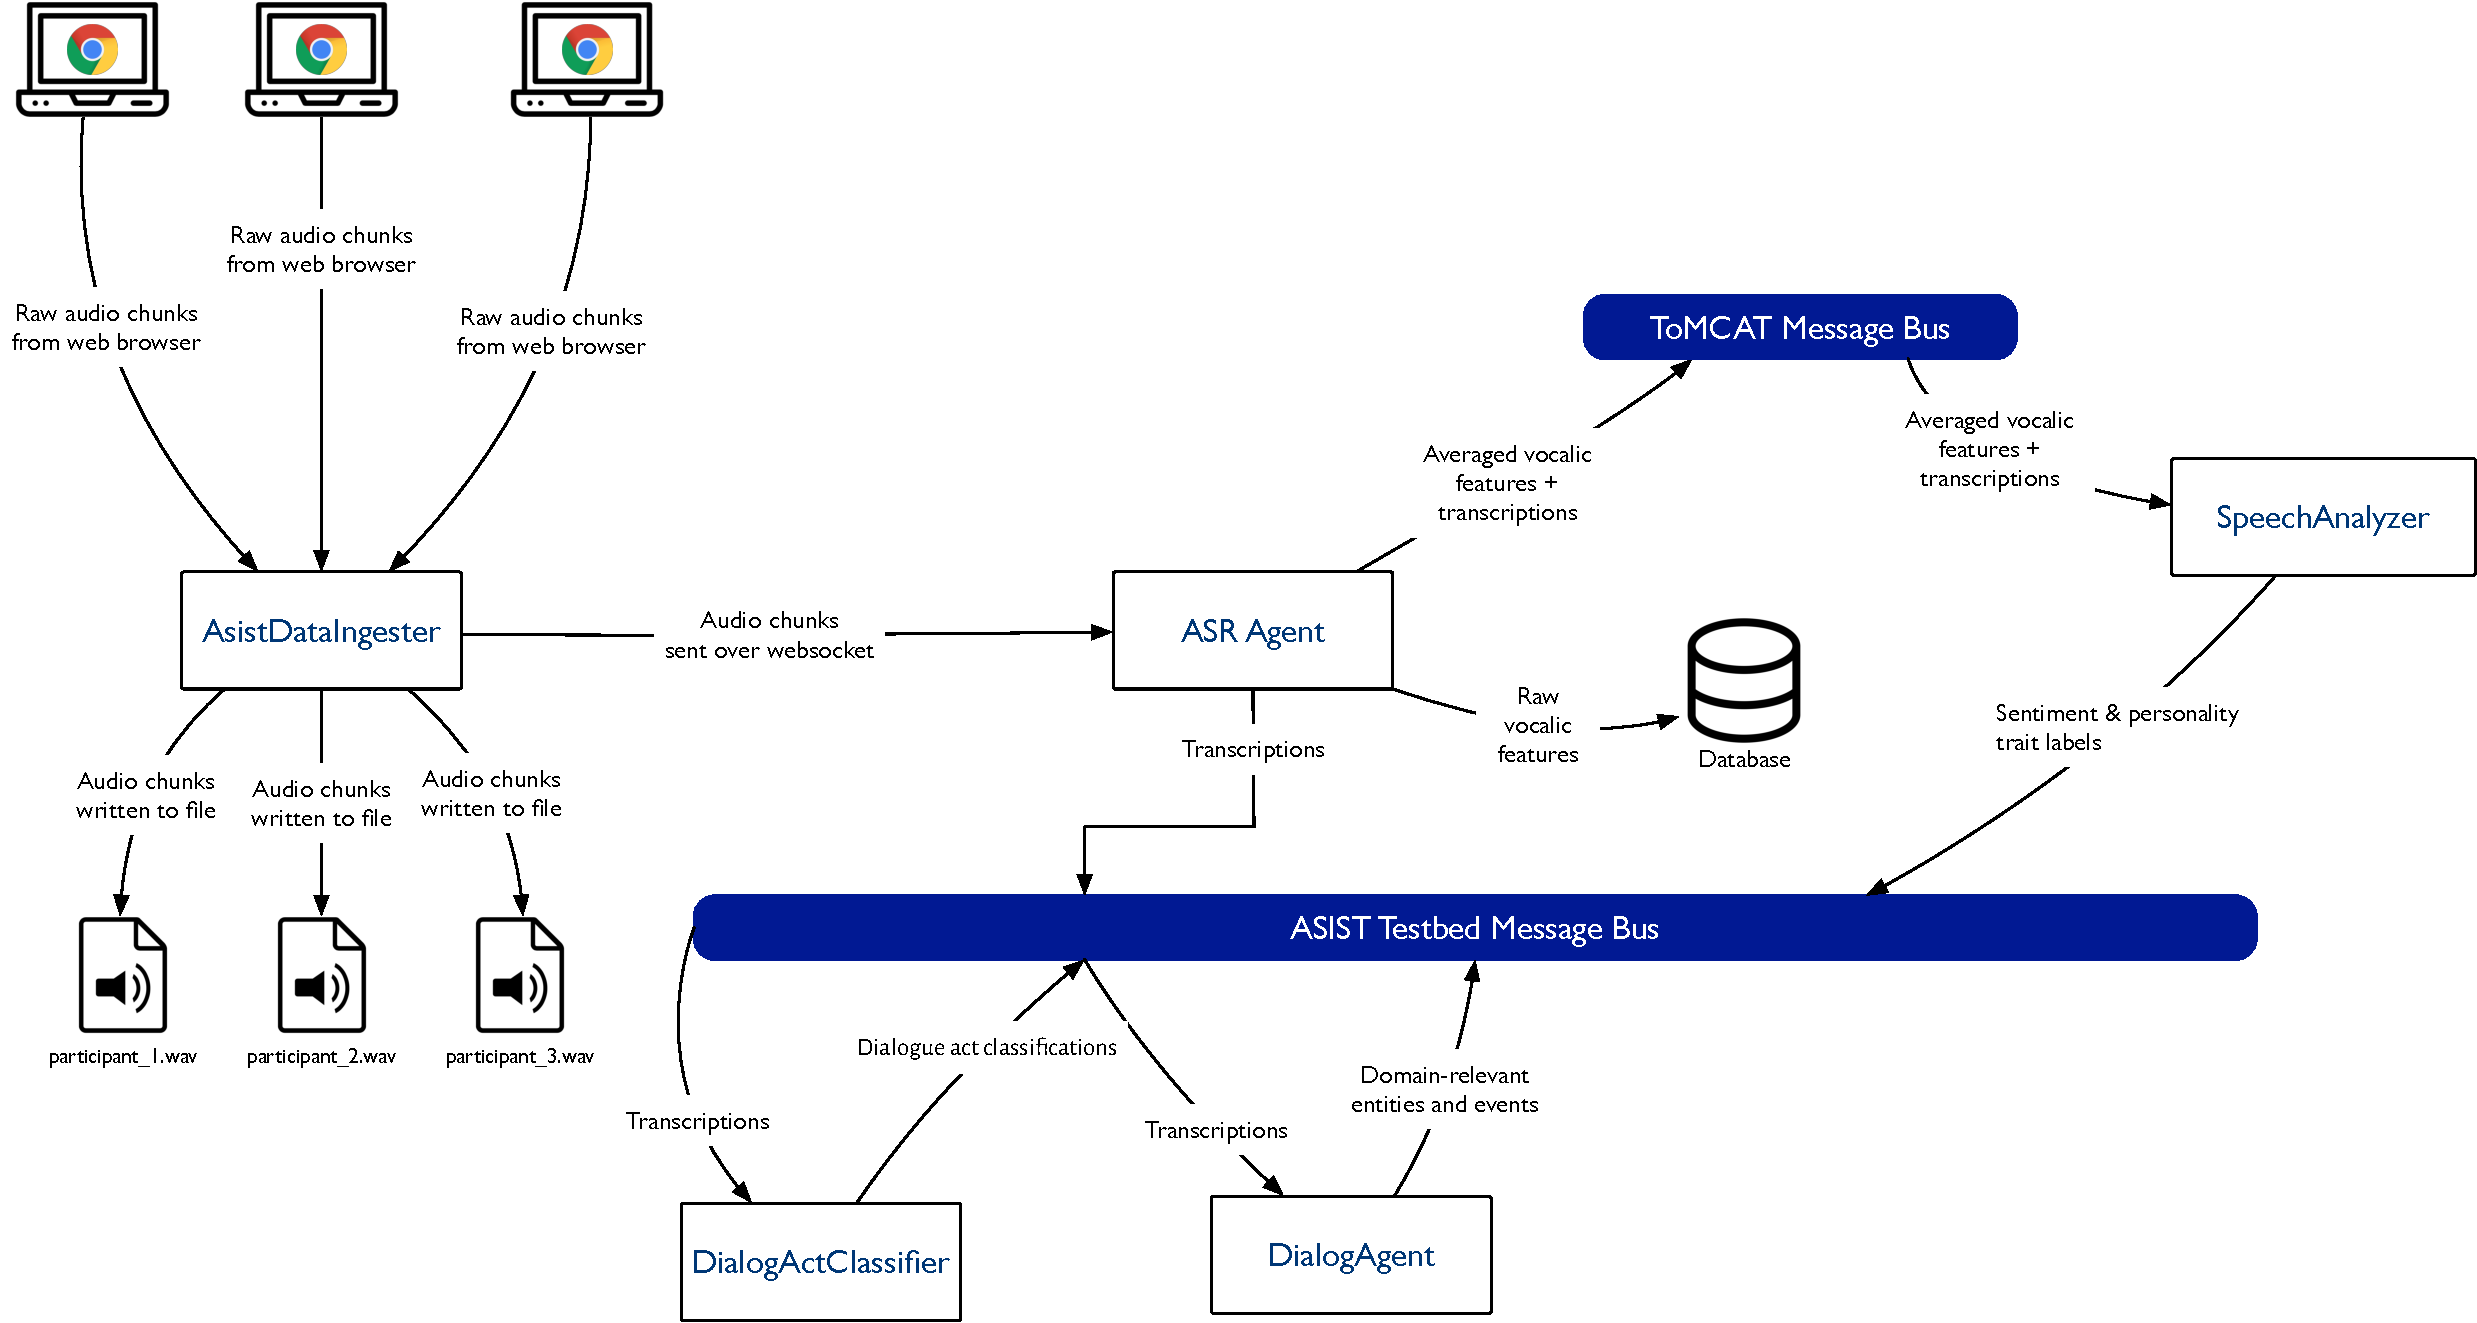
\includegraphics[width=6.5in]{images/nlp_architecture}
    \caption{Architecture of our multi-participant dialogue analysis system.}
    \label{fig:nlp-architecture}
\end{figure}

%Give a brief summary of the preregistrations and how they contribute to the overall architecture.

The component preregistrations in this document span a broad spectrum of
research topics, but work together to form a cohesive suite of ASI
capabilities.

Chapters \ref{ch:rule_based_ie} and \ref{ch:sentiment_analysis} focus on
gleaning information from individual natural language utterances. Chapter
\ref{ch:rule_based_ie} discusses our rule-based system for extracting entities
and events from natural language text, and \autoref{ch:sentiment_analysis}
describes our approach to detecting sentiment and personality traits using both
text and speech information.

In chapters \ref{ch:da_classification} and \ref{ch:clc}, we move
beyond analyzing utterances individually to analyzing them \emph{in context},
that is, we consider windows containing multiple utterances to detect
longer-range phenomena. Chapter \ref{ch:da_classification} uses context to identify
dialogue acts, and \autoref{ch:clc} uses it to automatically detect
closed-loop communication. Chapter \ref{ch:da_classification} also discusses
using multiple modalities (speech and text) to classify dialogue acts.

In \autoref{ch:entrainment}, we discuss our approach to detecting real-time
conversational alignment, or \emph{entrainment} between teammates. In
\autoref{ch:plan_recognition}, we describe our approach to multi-agent plan
recognition. The analyses described in this chapter will be performed offline
for ASIST Study 3, but we expect them to be integrated into online components
for ASIST Study 4 and future experiments.

Finally, we describe our probabilistic modeling approach to machine theory of
mind (MToM) and machine theory of teams (MToT) in \autoref{ch:pgm}, along with
our planned interventions in ASIST Study 3 and their rationale.
